\chapter{Evaluation}
\label{chap:07_evaluation}
%
\todo{Describe Chapter}

Möglich:
1. Effizienz Auto-Scaler
- Dynamisch skalieren vs statische Anzahl - > was ist schneller

2. GPU Worker
Ab wievielen statischen Worker mit CPU ONLY wird dieselbe Leistung erreicht

\section{Experimental Environment}
The experiments have been conducted on a NVIDIA DGX.
Table AB describes the hardware available on the DGX.
Two of the eight GPUs have been available to conduct the experiments.


The DGX is a live-system as being mentioned in Section XY. Therefore not all available hardware resource have been exclusively available to conduct these experiments.

\section{Workload}
% Intro
The performance evaluation of the implementation was conducted using two ML algorithms: K-Means and Naive Bayes.
% Implementation
To implement the algorithms, Apache Sparks ML library has been used. The K-Means implementation is available at ANHANG A and the Naive Bayes implementation at ANHANG B.


% Dataset
The \textit{infinite MNIST dataset}\cite{loosli2006InfiniteMNIST} has been used to to perform the algorithms. It consists of  8 million datapoints.


\subsection{K-Means}
K-Means is a unsupervised machine learning algorithm for clustering.
The algorithm aims to place unlabelled data, that appear to be related, into cluster.


In this section, we introduce perhaps the simplest unsupervised machine learning algorithms—k-means clustering. This algorithm analyzes unlabeled samples and attempts to place them in clusters that appear to be related. The k in “k-means” represents the number of clusters you’d like to see imposed on your data.The algorithm organizes samples into the number of clusters you specify in advance, using distance calculations similar to the k-nearest neighbors clustering algorithm. Each cluster of samples is grouped around a centroid—the cluster’s center point. Initially, the algorithm chooses k centroids at random from the dataset’s samples. Then the remaining samples are placed in the cluster whose centroid is the closest. The centroids are iteratively recalculated and the samples re-assigned to clusters until, for all clusters, the distances from a given centroid to the samples in its cluster are minimized. The algorithm’s results are:

\section{Efficiency of GPU Acceleration}


\section{Auto-Scaling using CPU Metrics}


\section{Results}
Ab wie viele worker ist CPU besser wie GPU

\begin{figure}[h]
\centering
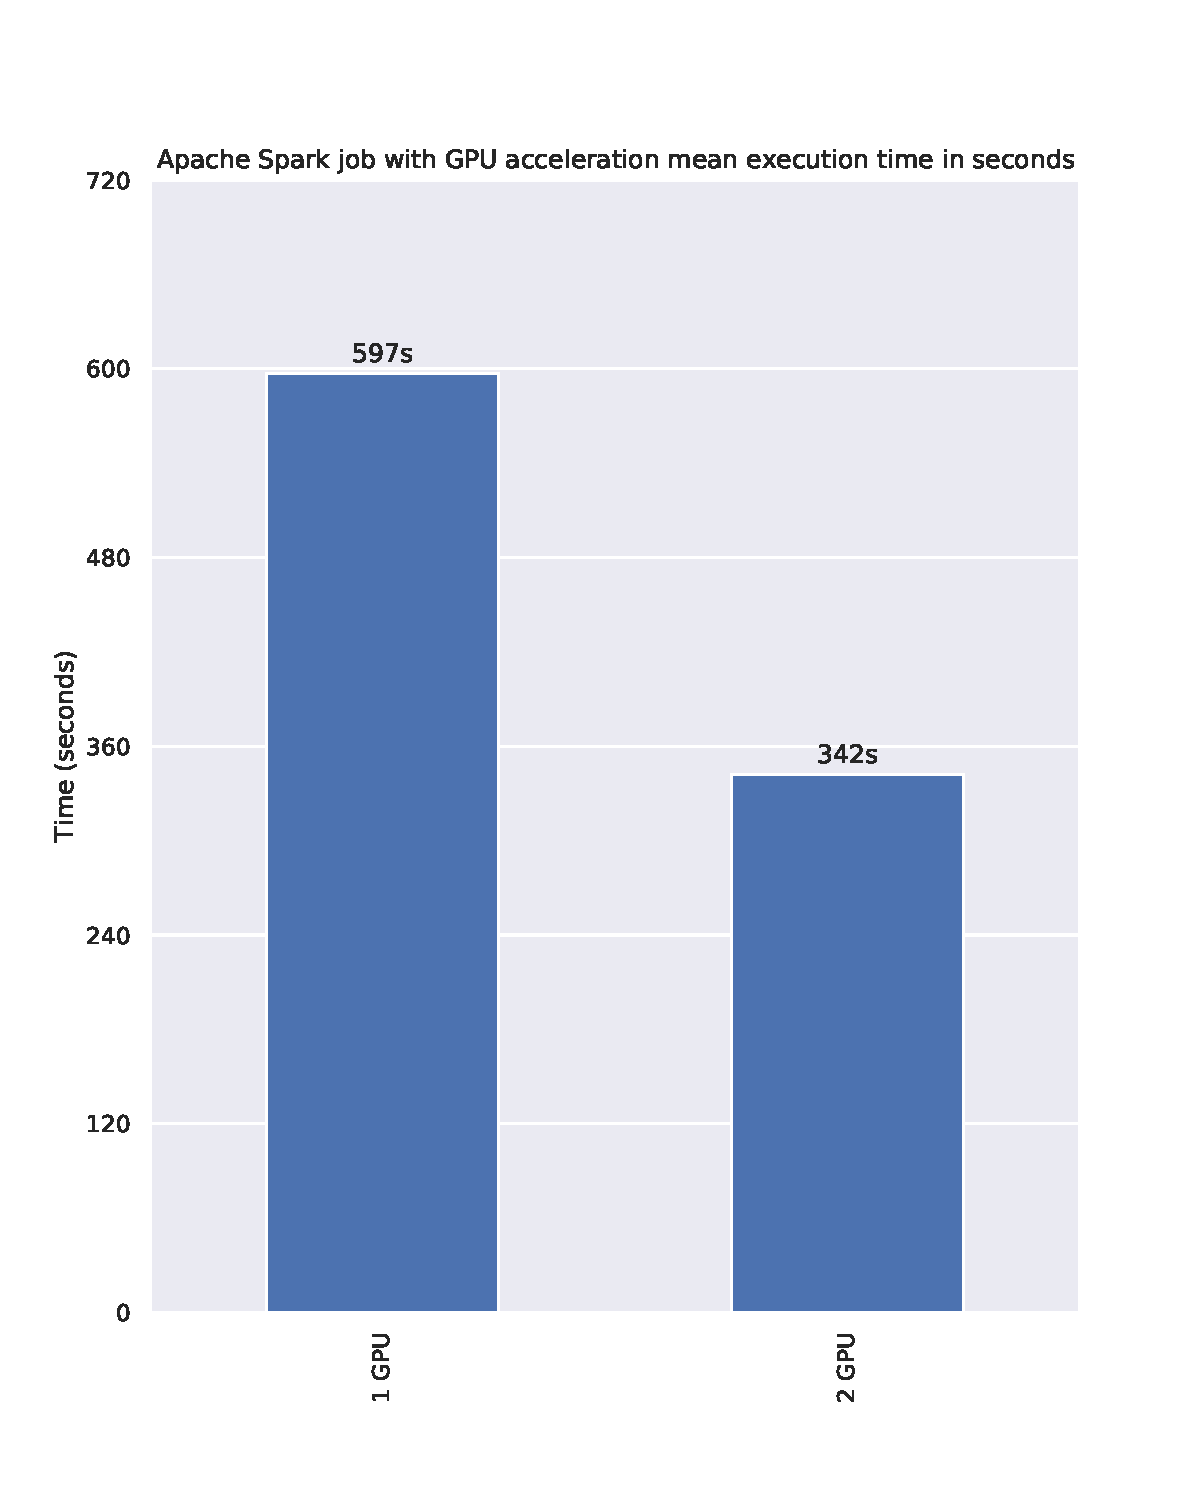
\includegraphics[scale=0.5]{images/07_evaluation/gpu_spark-job-mean-time}
\caption{Basic architecture of a GitLab CI/CD pipeline - Source: Authors own model, based on \cite{Gitlab2020Docs}.}
\label{fig:04_gitlab_pipeline_basic_arch}
\end{figure}

\begin{figure}[h]
\centering
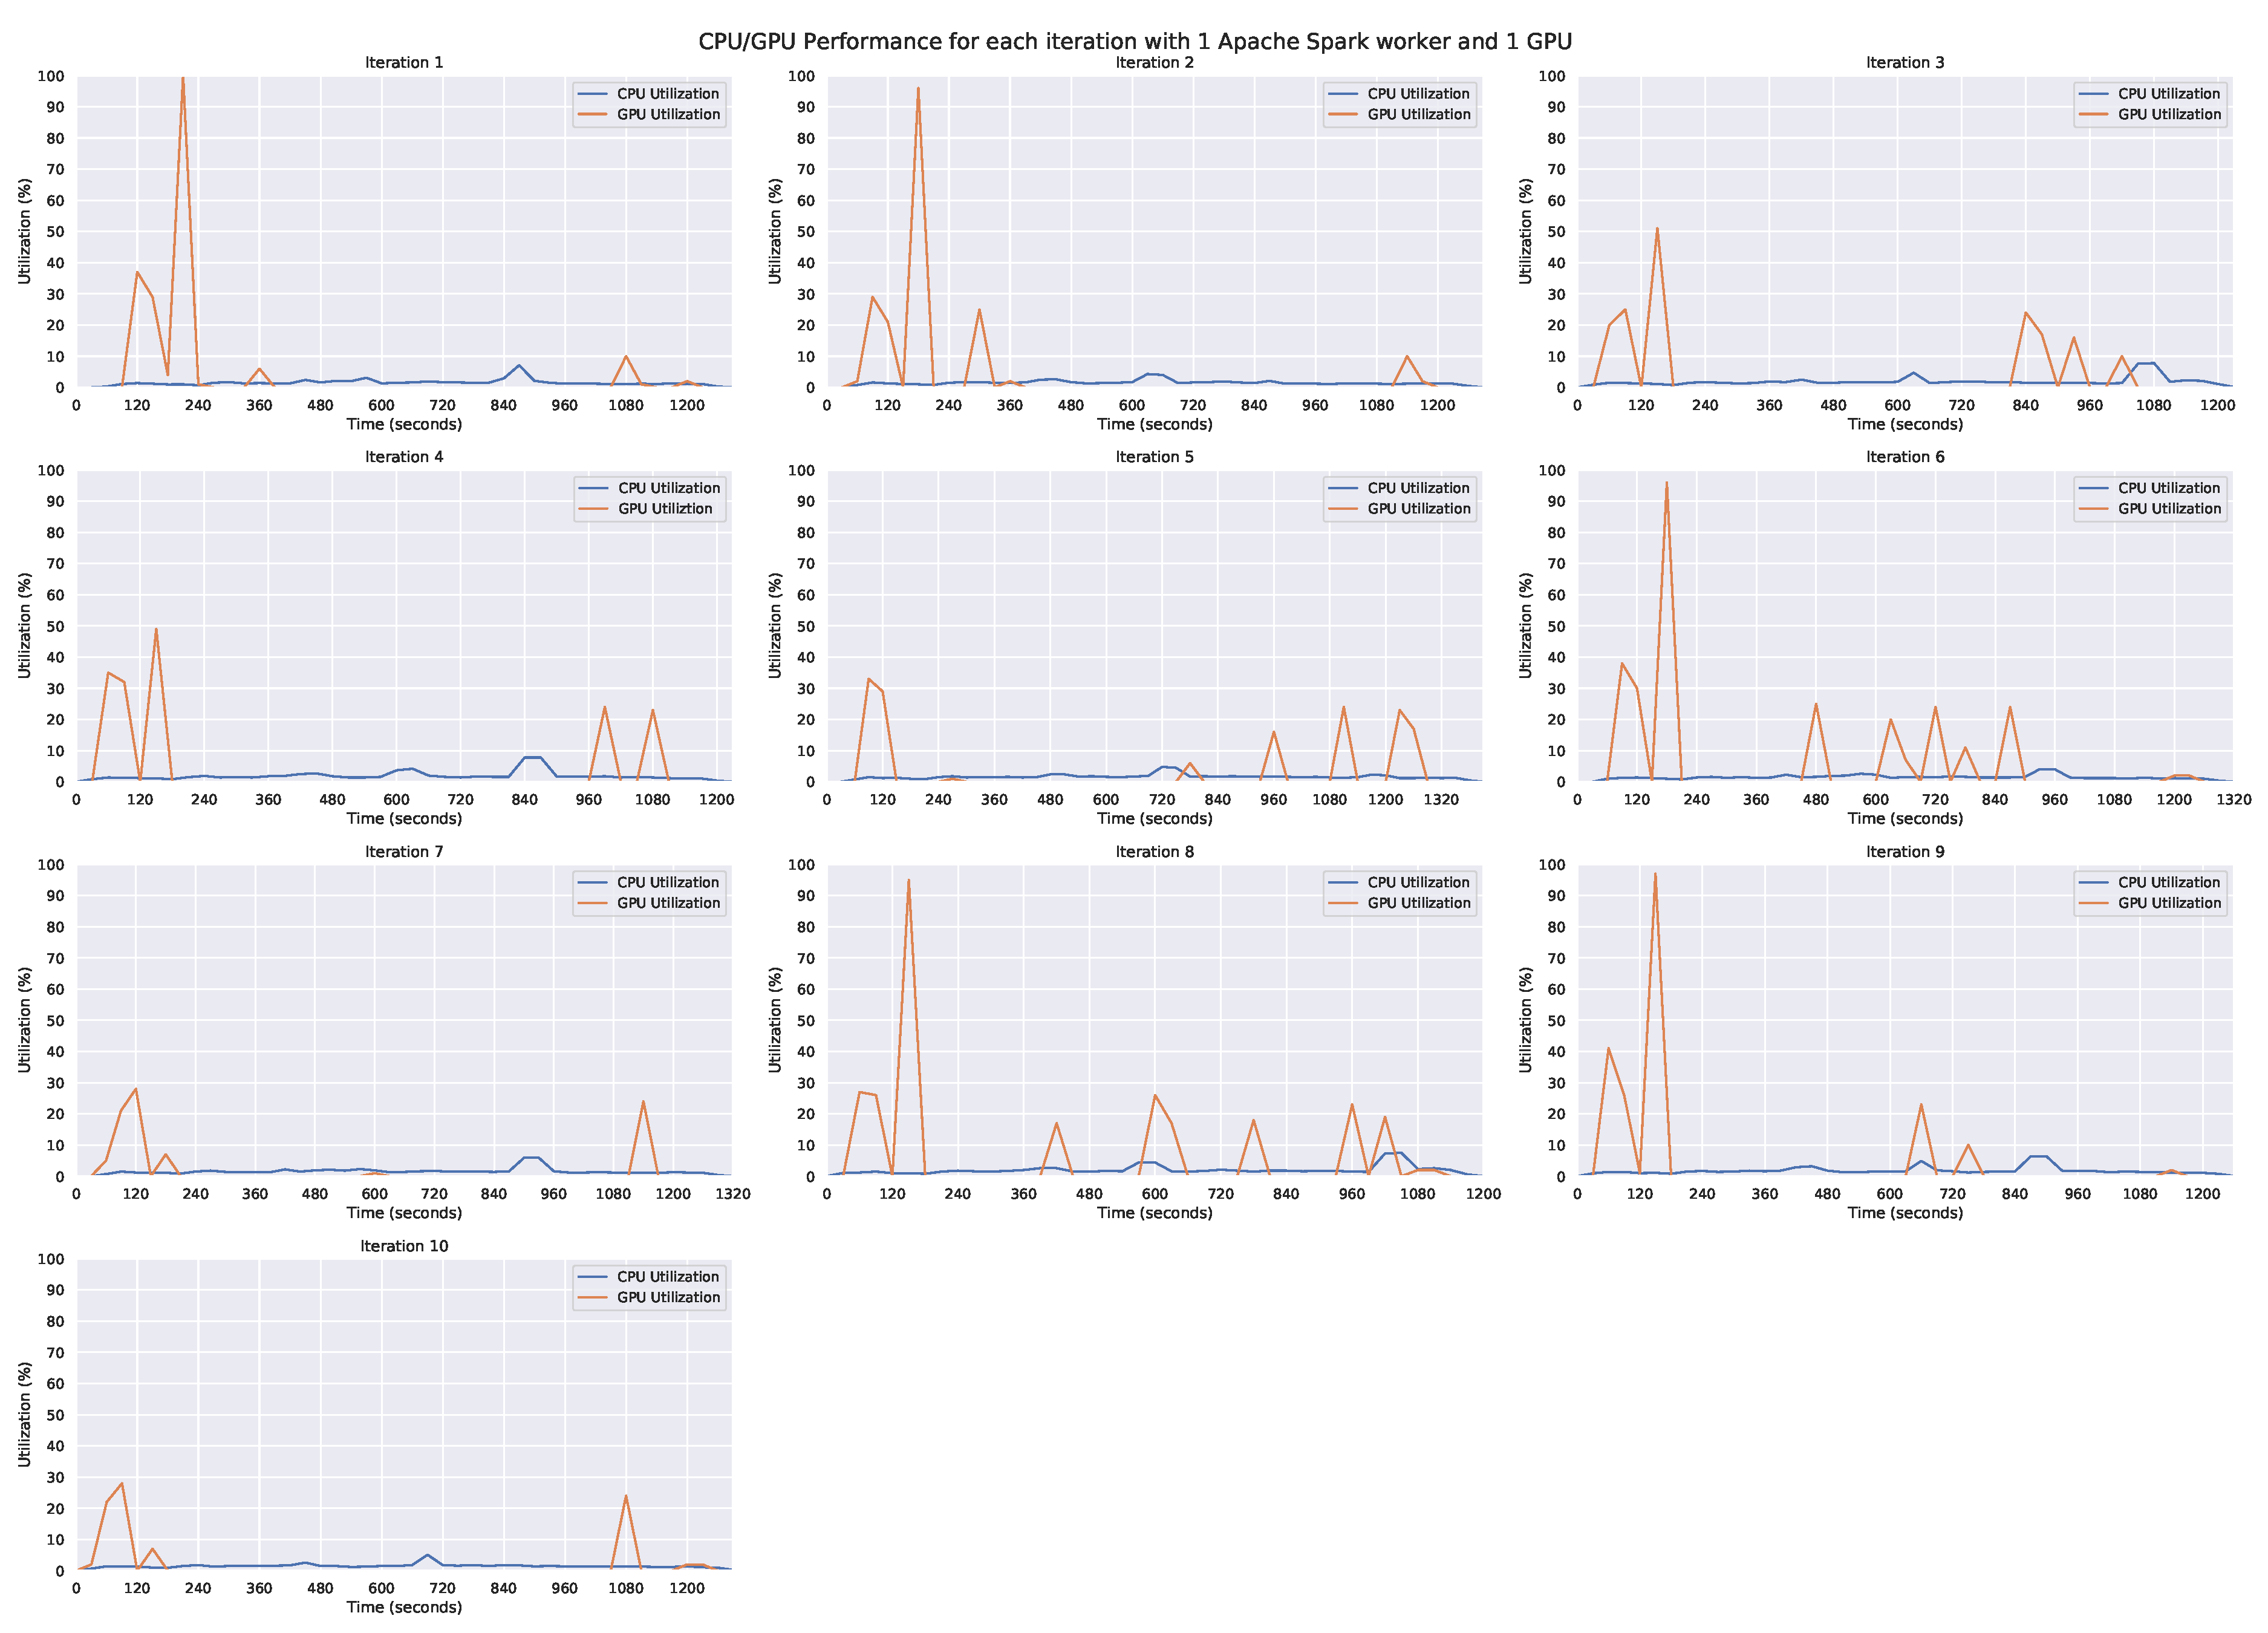
\includegraphics[scale=0.2]{images/07_evaluation/gpu1_performance}
\caption{Basic architecture of a GitLab CI/CD pipeline - Source: Authors own model, based on \cite{Gitlab2020Docs}.}
\label{fig:04_gitlab_pipeline_basic_arch}
\end{figure}
